\documentclass{article}

\usepackage{tikz} 
\usetikzlibrary{automata, positioning, arrows} 

\usepackage{amsthm}
\usepackage{amsfonts}
\usepackage{amsmath}
\usepackage{amssymb}
\usepackage{fullpage}
\usepackage{color}
\usepackage{parskip}
\usepackage{hyperref}
  \hypersetup{
    colorlinks = true,
    urlcolor = blue,
    linkcolor= blue,
    citecolor= blue,
    filecolor= blue,
    }
    
\usepackage{listings}
\usepackage[utf8]{inputenc}                                                    
\usepackage[T1]{fontenc}                                                       

\definecolor{dkgreen}{rgb}{0,0.6,0}
\definecolor{gray}{rgb}{0.5,0.5,0.5}
\definecolor{mauve}{rgb}{0.58,0,0.82}

\lstset{frame=tb,
  language=haskell,
  aboveskip=3mm,
  belowskip=3mm,
  showstringspaces=false,
  columns=flexible,
  basicstyle={\small\ttfamily},
  numbers=none,
  numberstyle=\tiny\color{gray},
  keywordstyle=\color{blue},
  commentstyle=\color{dkgreen},
  stringstyle=\color{mauve},
  breaklines=true,
  breakatwhitespace=true,
  tabsize=3
}

\newtheoremstyle{theorem}
  {\topsep}{\topsep}{\itshape\/}{0pt}{\bfseries}{.}{5pt plus 1pt minus 1pt}{}
\theoremstyle{theorem} 
   \newtheorem{theorem}{Theorem}[section]
   \newtheorem{corollary}[theorem]{Corollary}
   \newtheorem{lemma}[theorem]{Lemma}
   \newtheorem{proposition}[theorem]{Proposition}
\theoremstyle{definition}
   \newtheorem{definition}[theorem]{Definition}
   \newtheorem{example}[theorem]{Example}
\theoremstyle{remark}    
  \newtheorem{remark}[theorem]{Remark}

\setcounter{tocdepth}{3}
\setcounter{secnumdepth}{3}

\title{CPSC-354 Report}
\author{Jonathan Karam \\ Chapman University}

\date{\today} 

\begin{document}

\maketitle

\begin{abstract}
This report is a collection of notes, discussions, and homework solutions for CPSC 354. 
Homework 1 discusses the MIU puzzle and proves why \texttt{MI} cannot become \texttt{MU}. 
Homework 2 introduces abstract rewriting systems (ARS), includes TikZ diagrams, and classifies systems by termination, confluence, and unique normal forms. 
Homework 3 studies a rewriting system over $\{a,b\}$ and explores its equivalence classes and termination.
\end{abstract}

\tableofcontents

\section{Introduction}
This report documents my learning week by week. 
Each section includes my notes and discussions of the lecture topics, followed by my homework solutions.
The purpose is to show understanding, practice writing in \LaTeX{}, and explain the material in my own words.

\section{Week 1: The MIU Puzzle}

\subsection{Notes and Discussion}
The first week introduced the MIU puzzle, created by Douglas Hofstadter. 
It is a formal system that begins with the word \texttt{MI} and has four rules. 
The puzzle asks whether it is possible to reach \texttt{MU}. 
This is important because it shows how formal systems can be analyzed with invariants, a key concept in logic and computer science.

\subsection{Homework}
\textbf{Rules:}
\begin{enumerate}
  \item If a string ends with \texttt{I}, add a \texttt{U}.
  \item If a string starts with \texttt{M}, double the part after \texttt{M}.
  \item Replace \texttt{III} with \texttt{U}.
  \item Remove \texttt{UU}.
\end{enumerate}

\textbf{Why \texttt{MI} cannot become \texttt{MU}:}  
Let $\#I(w)$ be the number of \texttt{I}'s in $w$. Initially $\#I(\texttt{MI})=1$. 
Each rule preserves $\#I(w) \pmod{3}$:
\begin{itemize}
  \item Rule 1: no effect.
  \item Rule 2: doubles the count, $1 \mapsto 2$, never $0 \pmod 3$.
  \item Rule 3: subtracts 3, same remainder.
  \item Rule 4: no effect.
\end{itemize}
Thus $\#I(w) \pmod{3}$ is invariant. Since \texttt{MU} has $\#I=0$, it cannot be reached.

\textbf{Deeper explanation:}  
The invariant argument proves that all reachable words have I-count $\equiv 1$ or $2 \pmod{3}$, never 0.  
The first letter $M$ never disappears, so all reachable words start with $M$.  
Another way: define a homomorphism $h(M)=0, h(U)=0, h(I)=1 \pmod 3$. 
Every rule preserves $h$, so $h(\texttt{MI})=1$ and $h(\texttt{MU})=0$. Contradiction.  

\section{Week 2: Abstract Rewriting Systems}

\subsection{Notes and Discussion}
This week focused on abstract rewriting systems . 
An ARS consists of a set $A$ and a relation $R$. 
We care about whether rewriting always stops, whether different rewrite paths can rejoin, and whether normal forms are unique. 
These ideas are important in programming languages, compilers, and theorem provers.

\subsection{Homework}
We drew diagrams and classified ARSs.

\subsubsection*{Examples}
\begin{tikzpicture}
  % Example 1
\end{tikzpicture}

\textbf{1: $A=\{\}, R=\{\}$} (empty system)


\begin{tikzpicture}
  \node[draw,circle] (a) at (0,0) {a};
\end{tikzpicture}

\textbf{2: $A=\{a\}, R=\{\}$}

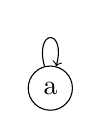
\begin{tikzpicture}
  \node[draw,circle] (a) at (0,0) {a};
  \draw[->] (a) to[loop above] (a);
\end{tikzpicture}

\textbf{3: $A=\{a\}, R=\{(a,a)\}$}

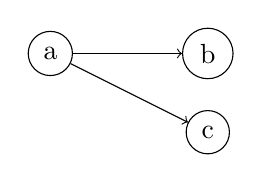
\begin{tikzpicture}
  \node[draw,circle] (a) at (0,0) {a};
  \node[draw,circle] (b) at (2,0) {b};
  \node[draw,circle] (c) at (2,-1) {c};
  \draw[->] (a) -- (b);
  \draw[->] (a) -- (c);
\end{tikzpicture}

\textbf{4: $A=\{a,b,c\}, R=\{(a,b),(a,c)\}$}

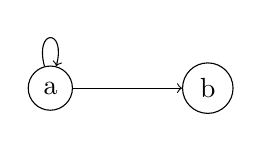
\begin{tikzpicture}
  \node[draw,circle] (a) at (0,0) {a};
  \node[draw,circle] (b) at (2,0) {b};
  \draw[->] (a) to[loop above] (a);
  \draw[->] (a) -- (b);
\end{tikzpicture}

\textbf{5: $A=\{a,b\}, R=\{(a,a),(a,b)\}$}

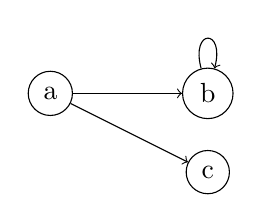
\begin{tikzpicture}
  \node[draw,circle] (a) at (0,0) {a};
  \node[draw,circle] (b) at (2,0) {b};
  \node[draw,circle] (c) at (2,-1) {c};
  \draw[->] (a) -- (b);
  \draw[->] (a) -- (c);
  \draw[->] (b) to[loop above] (b);
\end{tikzpicture}

\textbf{6: $A=\{a,b,c\}, R=\{(a,b),(b,b),(a,c)\}$}

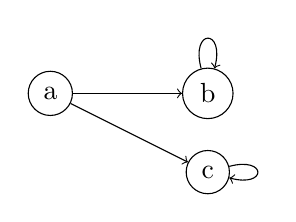
\begin{tikzpicture}
  \node[draw,circle] (a) at (0,0) {a};
  \node[draw,circle] (b) at (2,0) {b};
  \node[draw,circle] (c) at (2,-1) {c};
  \draw[->] (a) -- (b);
  \draw[->] (a) -- (c);
  \draw[->] (b) to[loop above] (b);
  \draw[->] (c) to[loop right] (c);
\end{tikzpicture}

\textbf{7: $A=\{a,b,c\}, R=\{(a,b),(b,b),(a,c),(c,c)\}$}

\subsubsection*{Classification Table}
\[
\begin{array}{c|c|c|c|l}
ARS & Terminating & Confluent & UN & Reason \\\hline
1 & Yes & Yes & Yes & Empty system \\
2 & Yes & Yes & Yes & a is normal \\
3 & No  & Yes & Yes & a \to a loop \\
4 & Yes & No  & No  & a \to b or c, two normals \\
5 & No  & Yes & Yes & all join at b \\
6 & No  & No  & Yes & a \to b (loop) or c (nf) \\
7 & No  & No  & Yes & no nfs, vacuous UN \\
\end{array}
\]

\section{Week 3: Strings over \{a,b\}}

\subsection{Notes and Discussion}
We studied rewriting rules over alphabet $\{a,b\}$. 
This shows how simple systems can classify strings into equivalence classes. 
We also saw how orienting rules one way can make a system terminating without changing equivalence.

\subsection{Homework 3}
\textbf{Exercise 5 rules:}
\[
ab \to ba,\quad ba \to ab,\quad aa \to \varepsilon,\quad b \to \varepsilon
\]

Examples: \texttt{abba} $\to$ \texttt{aa} $\to$ $\varepsilon$.  
\texttt{bababa} $\to$ \texttt{aaa} $\to$ \texttt{a}.  

Not terminating because swaps loop.  
Equivalence classes: even number of $a$’s $\to \varepsilon$, odd $\to a$.  
Normal forms: $\varepsilon, a$.  
Fix: orient $ba \to ab$ only.  

\textbf{Exercise 5b rules:}
\[
ab \leftrightarrow ba,\quad aa \to a,\quad b \to \varepsilon
\]

Examples: \texttt{abba} $\to$ \texttt{a}. \texttt{bababa} $\to$ \texttt{a}.  

Equivalence: all $b$ vanish, runs of $a$ collapse to one $a$.  
Classes: $\{\varepsilon,a\}$.  
Fix: orient swaps, keep $aa \to a$ and $b \to \varepsilon$.  

\section{Conclusion}
\textbf{Week 1:} Learned about invariants and why MU is impossible.  
\textbf{Week 2:} Saw ARS diagrams and how to classify systems.  
\textbf{Week 3:} Explored rewriting with $\{a,b\}$, equivalence classes, and how termination can be fixed.

\begin{thebibliography}{99}
\bibitem[BLA]{bla} Author, \href{https://en.wikipedia.org/wiki/LaTeX}{LaTeX Overview}, Publisher, Year.
\end{thebibliography}

\end{document}
